% fig_halow_signal_asymmetry.tex — Señal recibida y asimetría HaLow
% Datos: thesis_symmetric_package (Feb 2025, Laboratorio UNAL)
% v3 — Mejor alineación, tamaño adaptado a textwidth, leyenda reubicada
\begin{figure}[htbp]
\centering
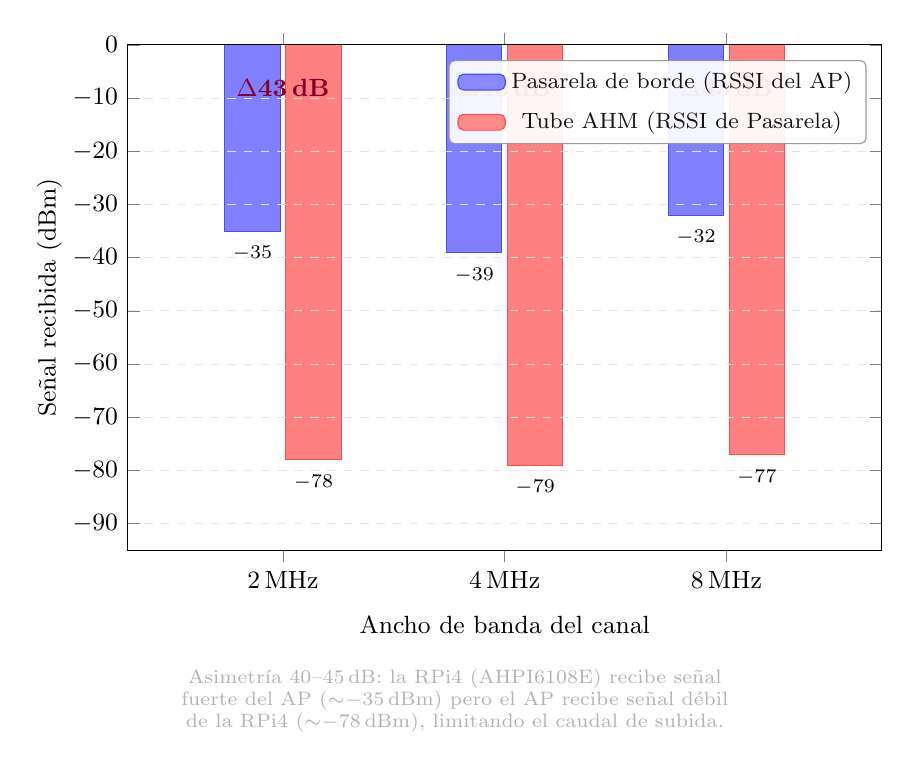
\begin{tikzpicture}
\begin{axis}[
    ybar,
    width=0.92\textwidth,
    height=8cm,
    bar width=20pt,
    enlarge x limits=0.35,
    ylabel={Se\~{n}al recibida (dBm)},
    ylabel style={font=\small, yshift=-3pt},
    xlabel={Ancho de banda del canal},
    xlabel style={font=\small, yshift=-3pt},
    symbolic x coords={2MHz, 4MHz, 8MHz},
    xtick=data,
    xticklabels={2\,MHz, 4\,MHz, 8\,MHz},
    xticklabel style={font=\small},
    ymin=-95, ymax=0,
    ytick={-90,-80,-70,-60,-50,-40,-30,-20,-10,0},
    yticklabel style={font=\small},
    legend style={at={(0.98,0.97)}, anchor=north east, legend columns=1, font=\footnotesize,
                  draw=black!40, fill=white, fill opacity=0.92, rounded corners=2pt,
                  row sep=3pt},
    nodes near coords,
    every node near coord/.append style={font=\scriptsize\bfseries, anchor=north, yshift=-2pt},
    ymajorgrids=true,
    major grid style={gray!20, dashed},
    tick label style={font=\small},
    label style={font=\small},
    axis on top,
    area legend,
    clip=false,
]

% Señal en Pasarela de borde (RPi4, medida del AP)
\addplot[fill=blue!50, draw=blue!70] coordinates {
    (2MHz, -35)
    (4MHz, -39)
    (8MHz, -32)
};

% Señal en Tube AHM (AP, medida de la Pasarela)
\addplot[fill=red!50, draw=red!70] coordinates {
    (2MHz, -78)
    (4MHz, -79)
    (8MHz, -77)
};

\legend{Pasarela de borde (RSSI del AP), Tube AHM (RSSI de Pasarela)}

% Anotaciones de asimetría (dentro del axis, coordenadas relativas)
\node[font=\small\bfseries, text=purple!70!black] at (axis cs:2MHz, -8) {$\Delta$43\,dB};
\node[font=\small\bfseries, text=purple!70!black] at (axis cs:4MHz, -8) {$\Delta$40\,dB};
\node[font=\small\bfseries, text=purple!70!black] at (axis cs:8MHz, -8) {$\Delta$45\,dB};

\end{axis}

% Nota explicativa con más espacio
\node[anchor=north, font=\scriptsize, text=gray!60, align=center, text width=0.85\textwidth] 
    at ([yshift=-6pt]current bounding box.south) {%
    Asimetr\'{i}a 40--45\,dB: la RPi4 (AHPI6108E) recibe se\~{n}al fuerte del AP ($\sim$$-$35\,dBm)
    pero el AP recibe se\~{n}al d\'{e}bil de la RPi4 ($\sim$$-$78\,dBm), limitando el caudal de subida.};

\end{tikzpicture}
\caption[Asimetr\'{i}a de se\~{n}al HaLow]{Se\~{n}al recibida (RSSI) y asimetr\'{i}a entre la pasarela de borde (RPi4 + AHPI6108E)
y el Tube AHM (puerta de malla) para cada ancho de banda del canal.
La diferencia de 40--45\,dB se atribuye a la mayor potencia de transmisi\'{o}n del Tube AHM
y explica la relaci\'{o}n 3--5$\times$ entre caudal de bajada y subida (Figura~\ref{fig:halow-tcp-throughput}).}
\label{fig:halow-signal-asymmetry}
\end{figure}
